\documentclass{article}
\usepackage{tikz}

\begin{document}

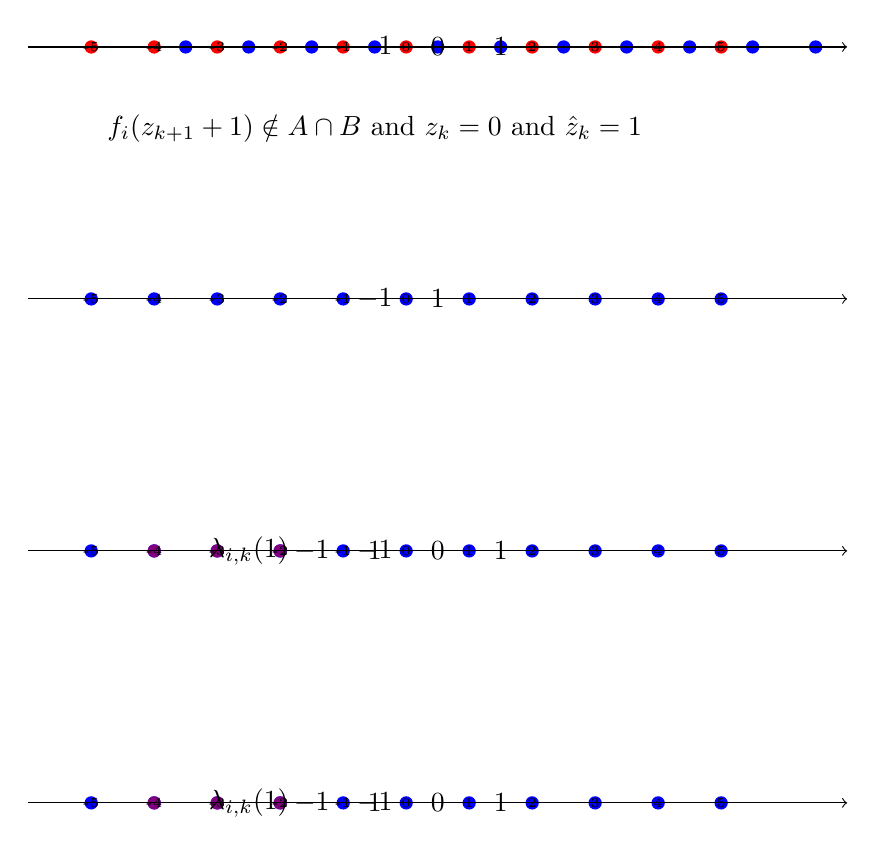
\begin{tikzpicture}[scale=0.8]
    \foreach \x in {-5,...,5}
    {
        \fill[red] (\x,-0.2) circle (3pt);
        \fill[blue] (\x+1.5,-0.2) circle (3pt);
    }
    
    \draw[->] (-6,-0.2) -- (7,-0.2);
    \foreach \x in {-5,...,5}
    {
        \node at (\x,-0.2) {\tiny \x};
    }
    
    \node at (-0.5,-0.2) {$-1$};
    \node at (0.5,-0.2) {$0$};
    \node at (1.5,-0.2) {$1$};

    \begin{scope}[yshift=-4cm]
        \foreach \x in {-5,...,5}
        {
            \fill[blue] (\x,-0.2) circle (3pt);
        }
        
        \draw[->] (-6,-0.2) -- (7,-0.2);
        \foreach \x in {-5,...,5}
        {
            \node at (\x,-0.2) {\tiny \x};
        }
        
        \node at (-0.5,-0.2) {$-1$};
        \node at (0.5,-0.2) {$1$};
    \end{scope}
    
    \begin{scope}[yshift=-8cm]
        \foreach \x in {-5,...,5}
        {
            \fill[blue] (\x,-0.2) circle (3pt);
        }
        \foreach \x in {-4,...,-2}
        {
            \fill[violet] (\x,-0.2) circle (3pt);
        }
        
        \draw[->] (-6,-0.2) -- (7,-0.2);
        \foreach \x in {-5,...,5}
        {
            \node at (\x,-0.2) {\tiny \x};
        }
        
        \node at (-0.5,-0.2) {$-1$};
        \node at (0.5,-0.2) {$0$};
        \node at (1.5,-0.2) {$1$};
        
        \node at (-2.5,-0.2) {$\lambda_{i,k}(1)$};
        \node at (-1.5,-0.2) {$-1$};
        \node at (-0.5,-0.2) {$1$};
    \end{scope}
    
    \begin{scope}[yshift=-12cm]
        \foreach \x in {-5,...,5}
        {
            \fill[blue] (\x,-0.2) circle (3pt);
        }
        \foreach \x in {-4,...,-2}
        {
            \fill[violet] (\x,-0.2) circle (3pt);
        }
        
        \draw[->] (-6,-0.2) -- (7,-0.2);
        \foreach \x in {-5,...,5}
        {
            \node at (\x,-0.2) {\tiny \x};
        }
        
        \node at (-0.5,-0.2) {$-1$};
        \node at (0.5,-0.2) {$0$};
        \node at (1.5,-0.2) {$1$};
        
        \node at (-2.5,-0.2) {$\lambda_{i,k}(1)$};
        \node at (-1.5,-0.2) {$-1$};
        \node at (-0.5,-0.2) {$1$};
    \end{scope}
    
    \node at (-0.5, -1.5) {$f_i(z_{k+1}+1) \notin A \cap B$ and $z_k = 0$ and $\hat{z}_k = 1$};
    
\end{tikzpicture}

\end{document}